\section{Objetivos}

\begin{itemize}
    \item Diseñar y simular un \textbf{control de ratio de caudal} para los caudales \textbf{FT10} y \textbf{FT11} en \textbf{Simulink}.

    \item Obtener la función de transferencia del nivel del tanque \textbf{T-10}.

    \item Diseñar y simular un \textbf{control en cascada de nivel a caudal} para el tanque \textbf{T-10}, considerando el lazo secundario de caudal \textbf{FC10} y el lazo primario de nivel \textbf{LC10}.

    \item Evaluar la respuesta de los controladores a partir de las gráficas solicitadas y de los \textbf{parámetros de desempeño}: porcentaje de sobreimpulso, tiempo de establecimiento y error en estado estable.
\end{itemize}

\section{Trabajo prelaboratorio}

\subsection{Control de ratio de caudal}

\begin{enumerate}[label=\arabic*)]
    \item Simule un \textbf{control de ratio de caudal} para los caudales \textbf{FT10} y \textbf{FT11} en \textbf{Simulink}, de modo que el diagrama de bloques tenga una estructura similar a la mostrada en la \textbf{Figura~\ref{fig:ratio}}. Para ello, realice lo siguiente:
    \begin{enumerate}[label=\alph*.]
        \item Obtenga o utilice funciones de transferencia previas para los flujómetros \textbf{FT10} y \textbf{FT11}. Para \textbf{FT10}, considere como entrada \textbf{u} el porcentaje de apertura de válvula \textbf{FV10/EV11} y como salida \textbf{y} el caudal de agua. Para \textbf{FT11}, considere como entrada \textbf{u} el comando de frecuencia del \textbf{VFD20} o la referencia de velocidad del \textbf{G120}, y como salida \textbf{y} el caudal de agua.

        \item Utilice el bloque \textbf{LTI System} para insertar la \textbf{función de transferencia}. Sintonice el controlador \textbf{PID} de caudal \textbf{FC11}, considerando las siguientes \textbf{especificaciones de control}: porcentaje de sobreimpulso \(<10\%\), tiempo de establecimiento \(<20\) s y error en estado estable \(<1\%\). Configure la saturación de salida del controlador como \textbf{0--60 Hz} para \textbf{VFD20} o \textbf{0--100\%} para \textbf{G120}.

        \item Inserte en \textbf{Simulink} los siguientes bloques:
        \begin{itemize}
            \item \textbf{Repeating Sequence Stair}, para generar el porcentaje de apertura de la válvula \textbf{FV10/EV11} y el valor de \textbf{ratio deseado}, con un \textbf{Sample time} de \textbf{40s}. Considere que el caudal deseado máximo posible para \textbf{FT11} es \textbf{75 l/min}.
            \item \textbf{Product}, para calcular el setpoint de \textbf{FC11} a partir del producto entre el caudal de \textbf{FT10} y el ratio deseado.
            \item \textbf{Divide}, para calcular el ratio medido \textbf{FT11/FT10}.
        \end{itemize}

        \item Simule el control de ratio de caudal con \textbf{dos valores diferentes} \(0 < [v_1,v_2] < 100\) para el porcentaje de apertura de válvula \textbf{FV10/EV11} y \textbf{tres valores diferentes} \(0 < [r_1,r_2,r_3] < 2\) para el ratio deseado. Utilice un tiempo de simulación de \textbf{160 s} y un \textit{Fixed-step size} de \textbf{0.01} o menor.
    \end{enumerate}

\begin{figure}[H]
    \centering
    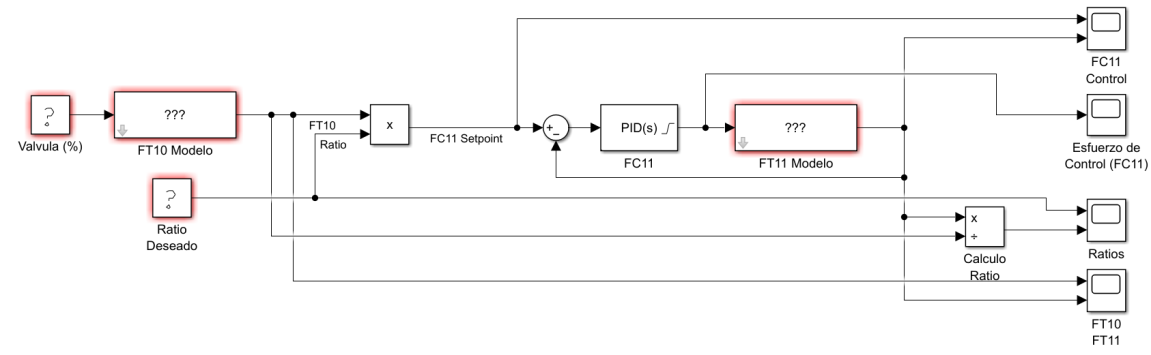
\includegraphics[width=\textwidth]{images/figure1.png}
    \caption{Diagrama de bloques en Simulink del control de ratio de caudal.}
    \label{fig:ratio}
\end{figure}

    \item Presente los siguientes resultados para el \textbf{control de ratio de caudal}:
    \begin{enumerate}[label=\alph*.]
        \item Funciones de transferencia utilizadas para \textbf{FT10} y \textbf{FT11}. Muestre el \textbf{porcentaje de estimación} correspondiente.
        \item Ganancias del controlador \textbf{PID FC11} obtenidas.
        \item Imagen del \textbf{diagrama de bloques} implementado en Simulink.
        \item Gráfica del control de caudal de \textbf{FT11}: setpoint de \textbf{FC11} vs. caudal medido de \textbf{FT11}.
        \item Parámetros de desempeño del control de \textbf{FT11}: porcentaje de sobreimpulso, tiempo de establecimiento y error en estado estable.
        \item Gráfica del esfuerzo de control de \textbf{FC11}: frecuencia del \textbf{VFD20} o porcentaje de velocidad del \textbf{G120}.
        \item Gráfica comparativa del \textbf{ratio}: ratio deseado vs. ratio medido.
        \item Gráfica comparativa de caudales: \textbf{FT10} vs. \textbf{FT11}.
    \end{enumerate}
\end{enumerate}

\subsection{Control en cascada de nivel a caudal}

\begin{enumerate}[label=\arabic*)]
    \item Simule un \textbf{control en cascada de nivel a caudal} para el nivel de agua del tanque \textbf{T-10} en \textbf{Simulink}, de modo que el diagrama de bloques tenga una estructura similar a la mostrada en la \textbf{Figura~\ref{fig:cascade}}. Para ello, realice lo siguiente:
    \begin{enumerate}[label=\alph*.]
        \item Obtenga o utilice una función de transferencia previa para el flujómetro \textbf{FT10}. Considere como entrada \textbf{u} el porcentaje de apertura de válvula \textbf{FV10/EV11} y como salida \textbf{y} el caudal de agua.

        \item Obtenga una función de transferencia para el medidor de nivel. Utilice \textbf{PT11/PT10} como señal de nivel, considere como entrada \textbf{u} el caudal de agua de entrada \textbf{FT10} y como salida \textbf{y} el porcentaje de nivel de agua del tanque. Muestre el \textbf{porcentaje de estimación} de la función identificada.

        \item Inserte y sintonice el controlador secundario \textbf{PID} de caudal \textbf{FC10}, considerando las siguientes \textbf{especificaciones de control}: porcentaje de sobreimpulso \(<10\%\), tiempo de establecimiento \(<20\) s y error en estado estable \(<1\%\). Configure la saturación de salida del controlador como \textbf{0--100\%} para \textbf{FV10} o \textbf{EV11}.

        \item Inserte controlador primario \textbf{PID} de nivel \textbf{LC10} de manera externa al controlador secundario, y sintonice. Considere las siguientes \textbf{especificaciones de control}: porcentaje de sobreimpulso \(<5\%\), tiempo de establecimiento \(<200\) s y error en estado estable \(<5\%\). Configure la saturación de salida del controlador como \textbf{0--17 l/min} para \textbf{Rockwell} o \textbf{0--35 l/min} para \textbf{Siemens}.

        \item Simule el control en cascada de nivel a caudal con un \textbf{setpoint de nivel de 50\%}. Utilice un tiempo de simulación de \textbf{300 s} y un \textit{Fixed-step size} de \textbf{0.01} o menor.
    \end{enumerate}

\begin{figure}[H]
    \centering
    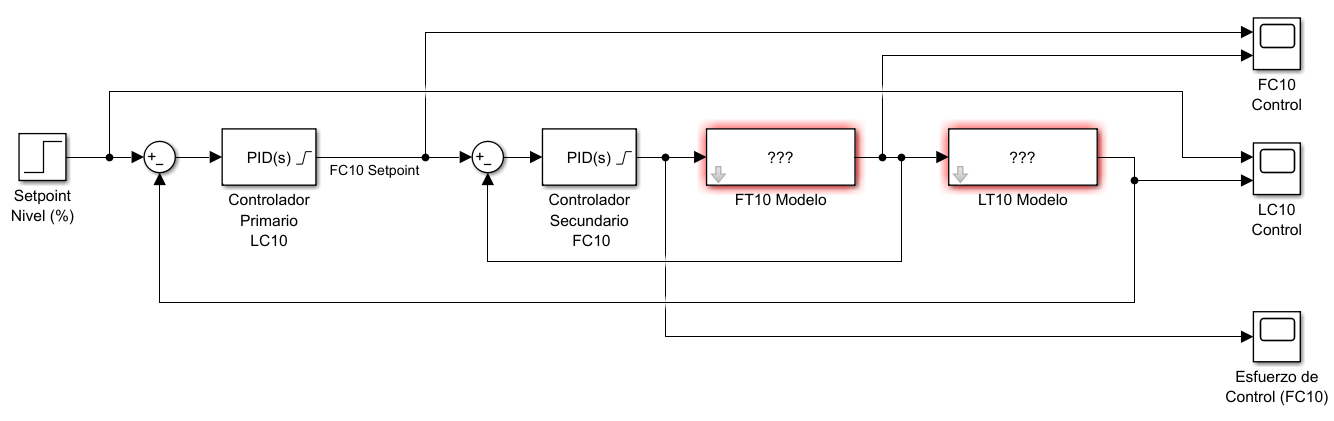
\includegraphics[width=\textwidth]{images/figure2.png}
    \caption{Diagrama de bloques en Simulink del control en cascada de nivel a caudal.}
    \label{fig:cascade}
\end{figure}

    \item Presente los siguientes resultados para el \textbf{control en cascada de nivel a caudal}:
    \begin{enumerate}[label=\alph*.]
        \item Funciones de transferencia utilizadas para \textbf{FT10} y para el nivel del tanque \textbf{T-10}, incluyendo el porcentaje de estimación del modelo de nivel.
        \item Ganancias de los controladores \textbf{PID FC10} y \textbf{LC10} obtenidas.
        \item Imagen del \textbf{diagrama de bloques} implementado en Simulink.
        \item Gráfica del control de caudal \textbf{FC10}: setpoint de caudal vs. caudal medido de \textbf{FT10}.
        \item Gráfica del control de nivel \textbf{LC10}: setpoint de nivel vs. nivel medido del tanque \textbf{T-10}.
        \item Gráfica del esfuerzo de control de \textbf{FC10}: porcentaje de apertura de \textbf{FV10/EV11}.
        \item Parámetros de desempeño del control de \textbf{FT10}: porcentaje de sobreimpulso, tiempo de establecimiento y error en estado estable.
        \item Parámetros de desempeño del control de nivel \textbf{LC10}: porcentaje de sobreimpulso, tiempo de establecimiento y error en estado estable.
    \end{enumerate}
\end{enumerate}
